%%%%%%%%%%%%%%%%%%%%%%%%%%%%%%%%%%%%%%%%%
%
% (c) 2019 by Jennifer Laaser
%
% This work is licensed under the Creative Commons Attribution-NonCommercial-ShareAlike 4.0 International License. To view a copy of this license, visit http://creativecommons.org/licenses/by-nc-sa/4.0/ or send a letter to Creative Commons, PO Box 1866, Mountain View, CA 94042, USA.
%
% The current source for these materials is accessible on Github: https://github.com/jlaaser/pogil-polymers
%
%%%%%%%%%%%%%%%%%%%%%%%%%%%%%%%%%%%%%%%%%

\renewcommand{\figpath}{content/polymphys/chain-confs/chain-elasticity/figs}
\renewcommand{\labelbase}{chain-elasticity}

\begin{activity}{Elasticity of Polymer Chains}

\begin{instructornotes}

	This activity introduces students to the concept of elasticity of polymer chains.
	
	After completing this activity, students will be able to:
			\begin{enumerate}
				\item Explain how the force to extend a chain is related to the free energy of the chain
				\item Explain what an ideal elastomer is, and identify situations in which a polymer might or might not be well-described as one
				\item Calculate the force required to extend a polymer chain under small deformations
				\item Explain why polymer chains are referred to as ``entropic springs''
			\end{enumerate}
	
			
	\subsection*{Activity summary:}
	\begin{itemize}
		\item \textbf{Activity type:} Learning Cycle
		\item \textbf{Content goals:} Basics of Chain Elasticity
		\item \textbf{Process goals:} %https://pogil.org/uploads/attachments/cj54b5yts006cklx4hh758htf-process-skills-official-pogil-list-2015-original.pdf
			\begin{itemize}
				\item Connecting key relationships to derive a result
				\item Interpreting mathematical equations in terms of physical behavior
				\item Oral and written communication of reasoning
			\end{itemize}
		\item \textbf{Duration:} approx. 50 minutes, including time for class discussion
		\item \textbf{Instructor preparation required:} 
			\begin{itemize}
				\item None beyond knowledge of relevant content
			\end{itemize}
		\item \textbf{Related textbook chapters:}
			\begin{itemize}
				\item \emph{Polymer Chemistry} (Hiemenz \& Lodge): Sections 6.7, 10.4, and 10.5.1
			\end{itemize}
	\end{itemize}

\end{instructornotes}

	%\textbf{Focus question:} Put a central question for the students to consider through this exercise here.

\begin{model}[Free Energy of Chain Stretching]
\label{\labelbase:mdl:delG}

	From basic thermodynamics, we know that the change in internal energy of a system during a process, $dU$, is
	\begin{equation*}
		dU = dq + dw
	\end{equation*}
	where $dq$ is the amount of heat transferred to the system and $dw$ is the amount of work done on the system.  We also know that the work done on a system is
	\begin{equation*}
		dw = f\,dL - P\,dV
	\end{equation*}
	where $f$ is the force acting on the material, $dL$ is the change in its length (the distance over which the force acts), $P$ is pressure, and $dV$ is change in volume.
	
	Using these relationships (see Exercise \ref{\labelbase:exc:dG}), it is possible to show that the change in Gibbs free energy is
	\begin{equation*}
		dG = f\,dL + V\,dP - S\,dT
	\end{equation*}
	where $S$ is entropy and $dT$ is change in temperature.

\end{model}


\begin{ctqs}

	\question Recall that for a function of three variables, $f(x,y,z)$, we can write
		\begin{equation*}
			df = \left(\frac{\partial f}{\partial x}\right)_{y,z}dx + 
				\left(\frac{\partial f}{\partial y}\right)_{x,z}dy +
				\left(\frac{\partial f}{\partial z}\right)_{x,y}dz
		\end{equation*}
		Write an analogous expression for $dG$, assuming that G is a function of pressure ($P$), temperature ($T$), and the length $L$ of the material.
		
		\begin{solution}[1in]\instructordisplay{
			\begin{equation*}
				dG = \left(\frac{\partial G}{\partial P}\right)_{T,L}dP + 
					\left(\frac{\partial G}{\partial T}\right)_{P,L}dT +
					\left(\frac{\partial G}{\partial L}\right)_{T,P}dL
			\end{equation*}
		}\end{solution}
		
	\question Compare your expression from the previous question to that given in Model 1.  What derivatives must each of the following values be equal to?
	
		\begin{enumerate}
			\item $f=$ \label{\labelbase:ctq:fderiv}
				\begin{solution}[0.5in]
					$f = \left(\frac{\partial G}{\partial L}\right)_{T,P}$
				\end{solution}
			\item $V=$
				\begin{solution}[0.5in]
					$\left(\frac{\partial G}{\partial P}\right)_{T,L}$
				\end{solution}
			\item $S=$
				\begin{solution}[0.5in]
					$S=  -\left(\frac{\partial G}{\partial T}\right)_{P,L}$ (note the negative sign)
				\end{solution}
		\end{enumerate}
		
	\question Recall that $G = H - TS$, where $H$ is the enthalpy of the material.  
	
		Substitute this expression into your answer to CTQ \ref{\labelbase:ctq:fderiv} and simplify to obtain an expression for $f$ in terms of $\left(\frac{dH}{dL}\right)_{P,T}$ and $\left(\frac{dS}{dL}\right)_{P,T}$.  \emph{(Hint: for the $TS$ term, remember that $T$ is constant!)}
		
		\begin{solution}[1.5in]\instructordisplay{
			\begin{align*}
				f &= \left(\frac{\partial G}{\partial L}\right)_{T,P}\\
					&= \left(\frac{\partial}{\partial L}(H-TS)\right)_{T,P}\\
					&= \left(\frac{\partial H}{\partial L}\right)_{T,P} - T\left(\frac{\partial S}{\partial L}\right)_{T,P}
			\end{align*}
		}\end{solution}
		
		\label{\labelbase:ctq:fdSdL}
	
\end{ctqs}

\begin{infobox}
	
	For simplicity, we will consider only \emph{ideal elastomers}.
	
	An ideal elastomer is a material in which there is no significant change in the enthalpy with changes in length.
	
\end{infobox}

\begin{ctqs}

	\question Using this information, write an expression for $f$ only in terms of the temperature, $T$, entropy, $S$, and length of the sample, $L$.
		
		\begin{solution}[0.75in]\instructordisplay{
			\begin{align*}
				f = - T\left(\frac{\partial S}{\partial L}\right)_{T,P}
			\end{align*}
		}\end{solution}
	
	\question Determine whether or not each of the following systems is likely to behave as an ideal elastomer.  Briefly note your group's reasoning for each case.
	
		\begin{enumerate}
			\item A chain of polyethylene stretched past its contour length
			
				\emph{Hint: what is likely to start happening to the bond lengths and bond angles in this case?}
		
				\begin{solution}[0.75in]
					Not likely to be an ideal elastomer - as bond lengths and bond angles distort, enthalpy will increase.
				\end{solution}
				
			\item A chain of polystyrene pulled from its collapsed globule form to its extended form under water
			
				\emph{Hint: polystyrene is hydrophobic.}
		
				\begin{solution}[0.75in]
					Not likely to be an ideal elastomer - there will be an enthalpic cost to pull the hydrophobic repeat units out of the globule and hydrate them.  (Note: hydrophobic hydration also has a significant entropic component from the water molecules, but the enthalpic component is key for this question.)
				\end{solution}
			
			\item A chain of poly(n-butyl acrylate) stretched gently in a network of other poly(n-butyl acrylate) chains
		
				\begin{solution}[0.75in]
					Reasonably likely to be an ideal elastomer - it is not being stretched to the limit, and the environment of the monomers is not changing.
				\end{solution}
		\end{enumerate}	
	
	\question In 1-2 complete sentences, briefly summarize what must be true about (1) the bond lengths and bond angles of the polymer, and (2) the surrounding environment in order for a polymer to behave as an ideal elastomer.
		
		\begin{solution}[1.5in]
			For a polymer chain to behave as an ideal elastomer, it can't be stretched to the point where bond lengths and bond angles begin to distort - it will behave as an ideal elastomer for relatively small deformations only.  The polymer's environment must also be such that the monomers see relatively the same interactions with their environment before and after chain extension.
		\end{solution}

\end{ctqs}

\begin{model}[Stretching a Single Chain]
\label{\labelbase:mdl:chainstretch}
	To understand the force that it takes to stretch a polymer chain, we need to know something about how the entropy changes as we change the length of the polymer chain.
	
	Consider stretching a single polymer chain, as shown below:
	
	\vspace{6pt}
	\centerline{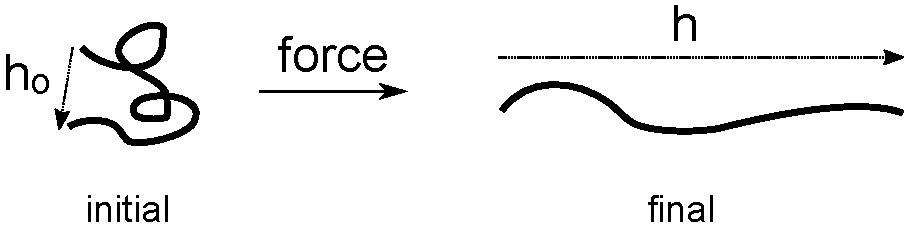
\includegraphics[width=0.55\textwidth]{\figpath/model2_chain-stretch.pdf}}
\end{model}

\begin{ctqs}
	\question Suppose that, in the initial state, the are $\Omega_i$ possible configurations of the chain that give end-to-end vector $\vec h_0$.  What is the entropy of this state?
	
		\emph{Hint: remember that $S = k\ln\Omega$.}
		
		\begin{solution}[0.25in]
			$S_i = k\ln\Omega_i$
		\end{solution}
	
	\question Suppose that in the final stretched state, there are $\Omega_f$ possible configurations of the chain that give end-to-end vector $\vec h$.  What is the entropy of this state?
		
		\begin{solution}[0.25in]
			$S_i = k\ln\Omega_f$
		\end{solution}
	
	\question Write an expression for the change in entropy that results from this stretching process, $\Delta S$, in terms of $\Omega_i$ and $\Omega_f$. \label{\labelbase:ctq:delS}
		
		\begin{solution}[0.75in]
			$\Delta S = S_f - S_i = k\ln\Omega_f - k\ln\Omega_i = k\ln\frac{\Omega_f}{\Omega_i}$
		\end{solution}
	
\end{ctqs}

\begin{infobox}

	As you have learned, the conformations of flexible polymer chains can be described as a random walk.
	
	For a polymer chain with $N$ monomers with statistical segment length $b$, the number of conformations giving end-to-end vector $\vec h$ is
	\begin{equation*}
		\Omega(\vec h) = A e^{-3h^2/2Nb^2}
	\end{equation*}
	where $A$ is a proportionality constant and $h$ is the end-to-end distance.
	
	Combining this expression with your answer to CTQ \ref{\labelbase:ctq:delS}, it is possible to show that the entropy change for a chain extended from end-to-end vector $\vec h_0$ to end-to-end vector $\vec h$ is
	\begin{equation*}
		\Delta S = \frac{3 k}{2 Nb^2}\left( h_0^2 - h^2 \right)
	\end{equation*}
	
\end{infobox}

\begin{ctqs}
	
	\question Since $h$ is essentially just the length of the chain, we can replace $L$ in the equation from CTQ \ref{\labelbase:ctq:fdSdL} with $h$ to obtain
		\begin{equation*}
			f = -T\left(\frac{d\Delta S}{dh}\right)
		\end{equation*}
		Using this expression, evaluate the force $f$ that it takes to stretch the chain to length $h$.
		\label{\labelbase:forcechain}
		
		\begin{solution}[2.5in]\instructordisplay{
			\begin{align*}
				f &= -T\left(\frac{d\Delta S}{dh}\right) \\
				  &= -T\left(\frac{d}{dh} \frac{3 k}{2 Nb^2}\left( h_0^2 - h^2 \right) \right) \\
				  &= -T \frac{3 k}{2 Nb^2} \left(\frac{d}{dh} \left( h_0^2 - h^2 \right) \right) \\
				  &= \frac{-3 k T}{2 Nb^2} (-2h)\\
				  &= \frac{3 k T}{Nb^2} h
			\end{align*}
		}\end{solution}
		
	\question Compare your result to the following expression for the force required to extend a spring to length $x$:
		\begin{equation*}
			F = kx
		\end{equation*}
		(As you may recall from physics, this equation is \emph{Hooke's Law}.)
		
		\begin{enumerate}
			\item Which variable in your answer to CTQ \ref{\labelbase:forcechain} is analogous to the length of the spring, $x$?
		
				\begin{solution}[0.75in]
					$h$
				\end{solution}
			
			\item Which collection of variables in your answer to CTQ \ref{\labelbase:forcechain} gives the spring constant, $k$?
		
				\begin{solution}[0.75in]
					$\frac{3kT}{Nb^2}$
				\end{solution}
			
		\end{enumerate}
		
	\question Explain, in 2-3 complete sentences, why we often describe polymers as ``entropic springs.''
	
		\begin{solution}[2.5in]
			The force law for extending a polymer chain is analogous to Hooke's law, and it was derived from the entropic properties (configurations) of the polymer chains.  The force that ``pulls back'' when we pull on a polymer chain is entirely due to the entropic drive to favor the end-to-end distances with the highest number of polymer conformations giving that distance.  No enthalpic contribution is necessary to give rise to this spring-like behavior.
		\end{solution}
	
\end{ctqs}
	
	
\begin{exercises}
	\exercise \label{\labelbase:exc:dG} Derive the expression for $dG$ given in Model \ref{\labelbase:mdl:delG} by doing the following:
	
		\begin{enumerate}
			\item Recall that $H = U+ PV$, and $G=H-TS$.  Using this information, write an expression for the Gibbs free energy, $G$, in terms of $U$, $P$, $V$, $T$, and $S$.
			
				\begin{solution}\instructordisplay{
					\begin{align*}
						G &= H-TS \\
							&= U + PV - TS
					\end{align*}
				}\end{solution}
			
			\item Differentiate your expression from the previous part to find an expression for the total differential of the Gibbs free energy, $dG$.
			
				\emph{Hint: if it helps, you might find it useful to differentiate $G$ with respect to some arbitrary variable (say, $x$), and follow the product rule through assuming that $U$, $P$, $V$, $T$, and $S$ are all functions of that variable.  Then drop the $dx$ on the bottom of all of the derivatives to obtain an answer in the form of the total differential.}
			
				\begin{solution}\instructordisplay{
					\begin{align*}
						G = U + PV - TS
					\end{align*}
					so
					\begin{equation*}
						\frac{dG}{dx} = \frac{dU}{dx} + P\frac{dV}{dx} + V\frac{dP}{dx} - T\frac{dS}{dx} - S\frac{dT}{dx}
					\end{equation*}
					and
					\begin{equation*}
						dG = dU + P\,dV + V\,dP - T\,dS - S\,dT
					\end{equation*}
				}\end{solution}
				
			\item Finally, combine your result from the previous problem with the expressions for $dU$ and $dw$ given in Model \ref{\labelbase:mdl:delG} to obtain the desired expression for $dG$.  You will find it helpful to remember that heat flow is related to entropy by $dq = T dS$.
			
				\begin{solution}\instructordisplay{
					From the model, we know that $dU = dq + dw$ and $dw = f\,dL - p\,dV$.  Combining this with our previous result, and the information about $dq$ given in the problem, we obtain
					\begin{align*}
						dG &= dq + dw + P\,dV + V\,dP - T\,dS - S\,dT\\
						   &= T\,dS + f\,dL - P\,dV + P\,dV + V\,dP - T\,dS - S\,dT\\
						   &= f\,dL + (P\,dV - P\,dV) + V\,dP + (T\,dS - T\,dS) - S\,dT\\
						   &= f\,dL + V\,dP - S\,dT
					\end{align*}
				}\end{solution}
		\end{enumerate}

	\exercise If you increase the temperature of a polymeric material, do you expect it to become stiffer (more difficult to stretch) or softer (easier to stretch)?  Explain your reasoning in 1-2 complete sentences.
	
		\begin{solution}\instructordisplay{
			The material should become stiffer.  The effective spring constant for the polymer chains is proportional to temperature, so increasing temperature increases the spring constant.  Increasing the spring constant increases the amount of force that it takes to extend the material by the same amount, so we will perceive the material as becoming stiffer, or harder to extend.
		}\end{solution}
\end{exercises}
	
\end{activity}